\documentclass{beamer}
\usetheme{Berlin}
\usecolortheme{seahorse}

\usepackage{graphicx}
\usepackage{subcaption}

\title{Gravitationally lensed quasars in the JPAS survey}
\author{Alexey V. Sergeyev}
\date{\today}

\begin{document}

\frame{\titlepage}

\section{Introduction}
\begin{frame}
    \frametitle{How to looks gravitationally lensed quasars}
    \begin{columns}
        \column{0.5\textwidth}
        \only<1>{\begin{itemize}
            \item Separaion between quasar images 
            \begin{figure}
                \centering
                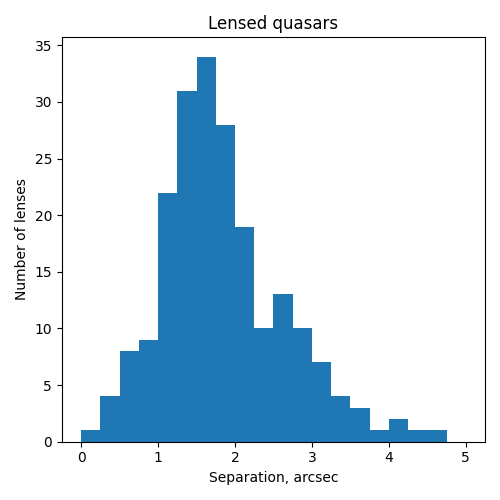
\includegraphics[width=0.8\textwidth]{../../figs/glq_separation_hist.png}
            \end{figure}
        \end{itemize}}

        \only<2>{\begin{itemize}
            \item Distribution of quasar images on the sky
            \begin{figure}
                \centering
                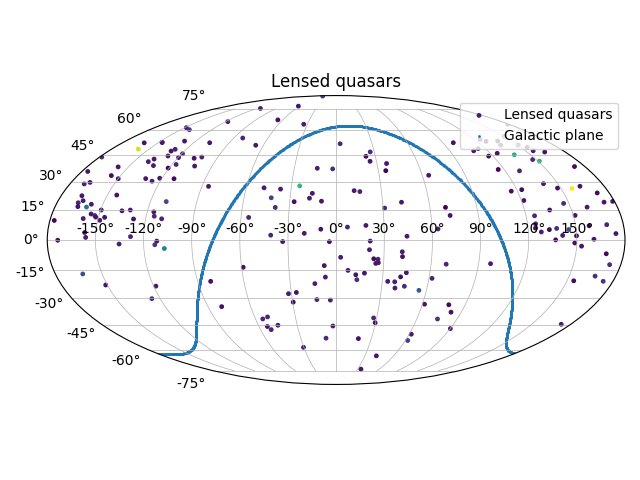
\includegraphics[width=0.8\textwidth]{../../figs/glq_sky_map.png}
            \end{figure}
        \end{itemize}}

        \only<3>{\begin{itemize}
            \item Distribution of quasar images on the sky
            \begin{figure}
                \centering
                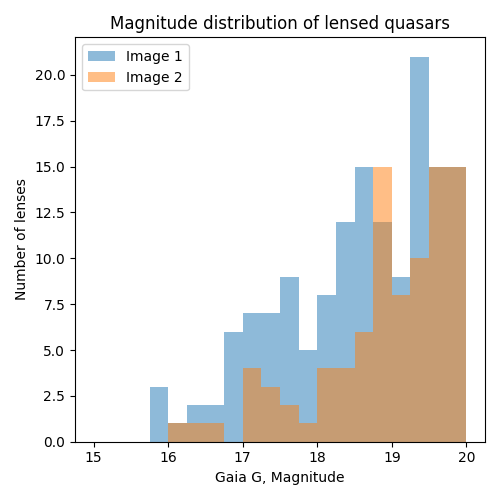
\includegraphics[width=0.8\textwidth]{../../figs/glq_mag_hist.png}
            \end{figure}

        \end{itemize}}
        \column{0.5\textwidth}
        \begin{figure}
            \centering
            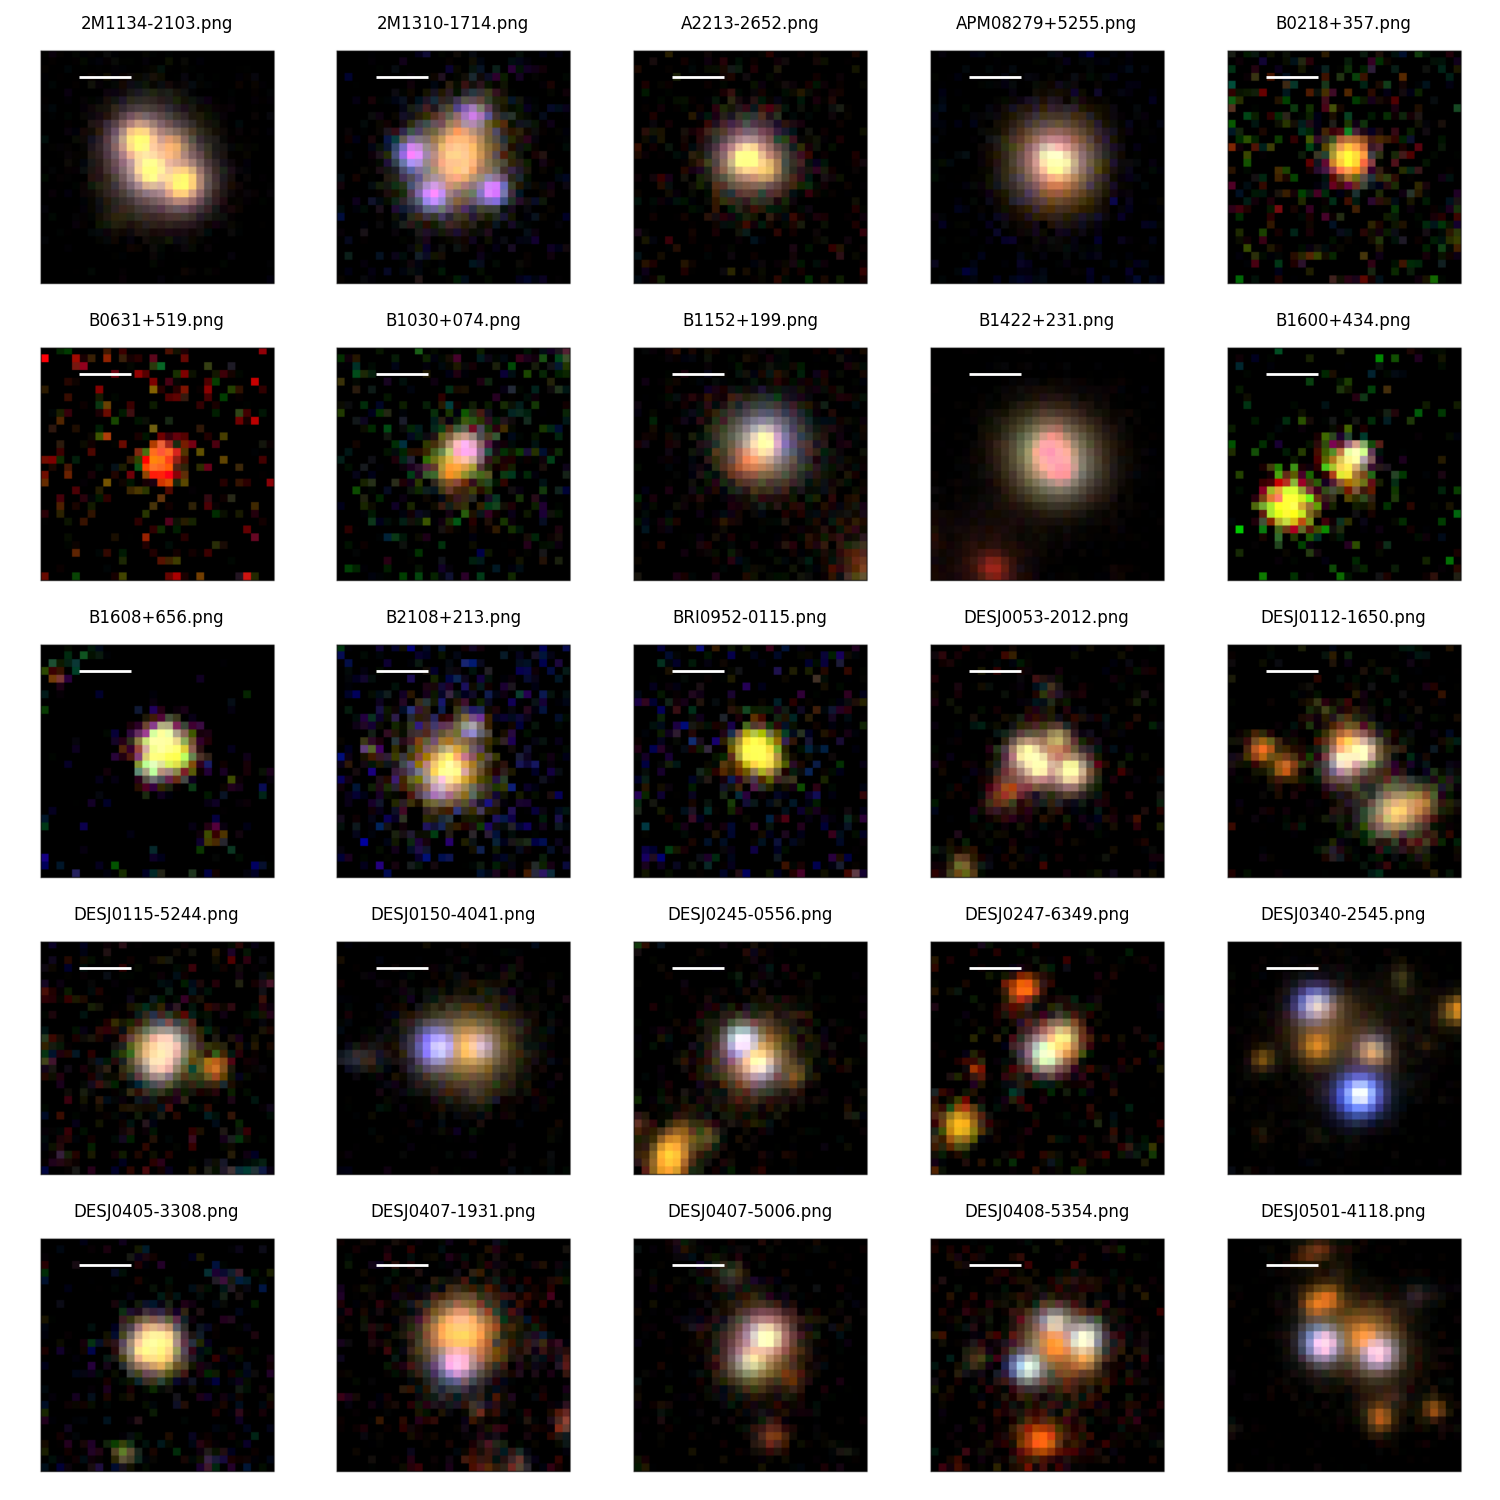
\includegraphics[width=1.0\textwidth]{../../figs/lensed_quasars.png}
            \caption{Gravitationally Lensed Quasar Database}
        \end{figure}
    \end{columns}

    \note{I would like to start with the general description of the gravitationally lensed sources information.
    How look gravitationally lensed quasars in survey data.
    How many gravitationally lensed quasars were found before, and how many we can find in the JPAS survey.
    Existing methods of finding gravitationally lensed quasars.
    Methods of finding gravitationally lensed galaxies.
    Technics of finding gravitationally lensed quasars and galaxies. 
    }
\end{frame}

\begin{frame}
\frametitle{The properties of gravitationally lensed quasars}
    \begin{itemize}
        \item Multiple point-like images (sep $\approx 2"$) 
        \item Presence of a lensing galaxy between the images
        \item Simmilary of the image colors (could be distorssed by the lensing galaxy)
    \end{itemize} 
\end{frame}

\section{Selection of candidates}
\begin{frame}
    \frametitle{Source selection}
    \begin{itemize}
        \item Source Quasar surveys: 
        SDSS:
        Advantages: have spectra (BOSS, e-BOSS etc.) 
        Disadvantages: Have a limited number of sources with measured. 

        GAIA sources: 
        Advantages: have a proper motion and parallax maeasurements,
        as well as precise spatial resolution. Have a large number of sources. The DR3 have a catalog of quasars.
        Disadvantages: Limited of magnitude (<=20), the only two bands (BP, RP) photometry (G band cover entire wavelenght range).

    \end{itemize}
\end{frame}

\section{SDSS sources}

\begin{frame}
    \frametitle{JPAS vs. SDSS spectra}
    \begin{columns}
        \column{0.5\textwidth}
        \begin{table}
            \caption{SDSS spectra in JPAS-mini}
            \centering
            \begin{tabular}{|c|c|}
                \hline
                Class & Number \\
                \hline
                    GALAXY   & 514 \\
                    STAR     & 238 \\
                    QSO      & 182 \\
                \hline
            \end{tabular}
        \end{table}
        \column{0.5\textwidth}
        \begin{figure}
            \centering
            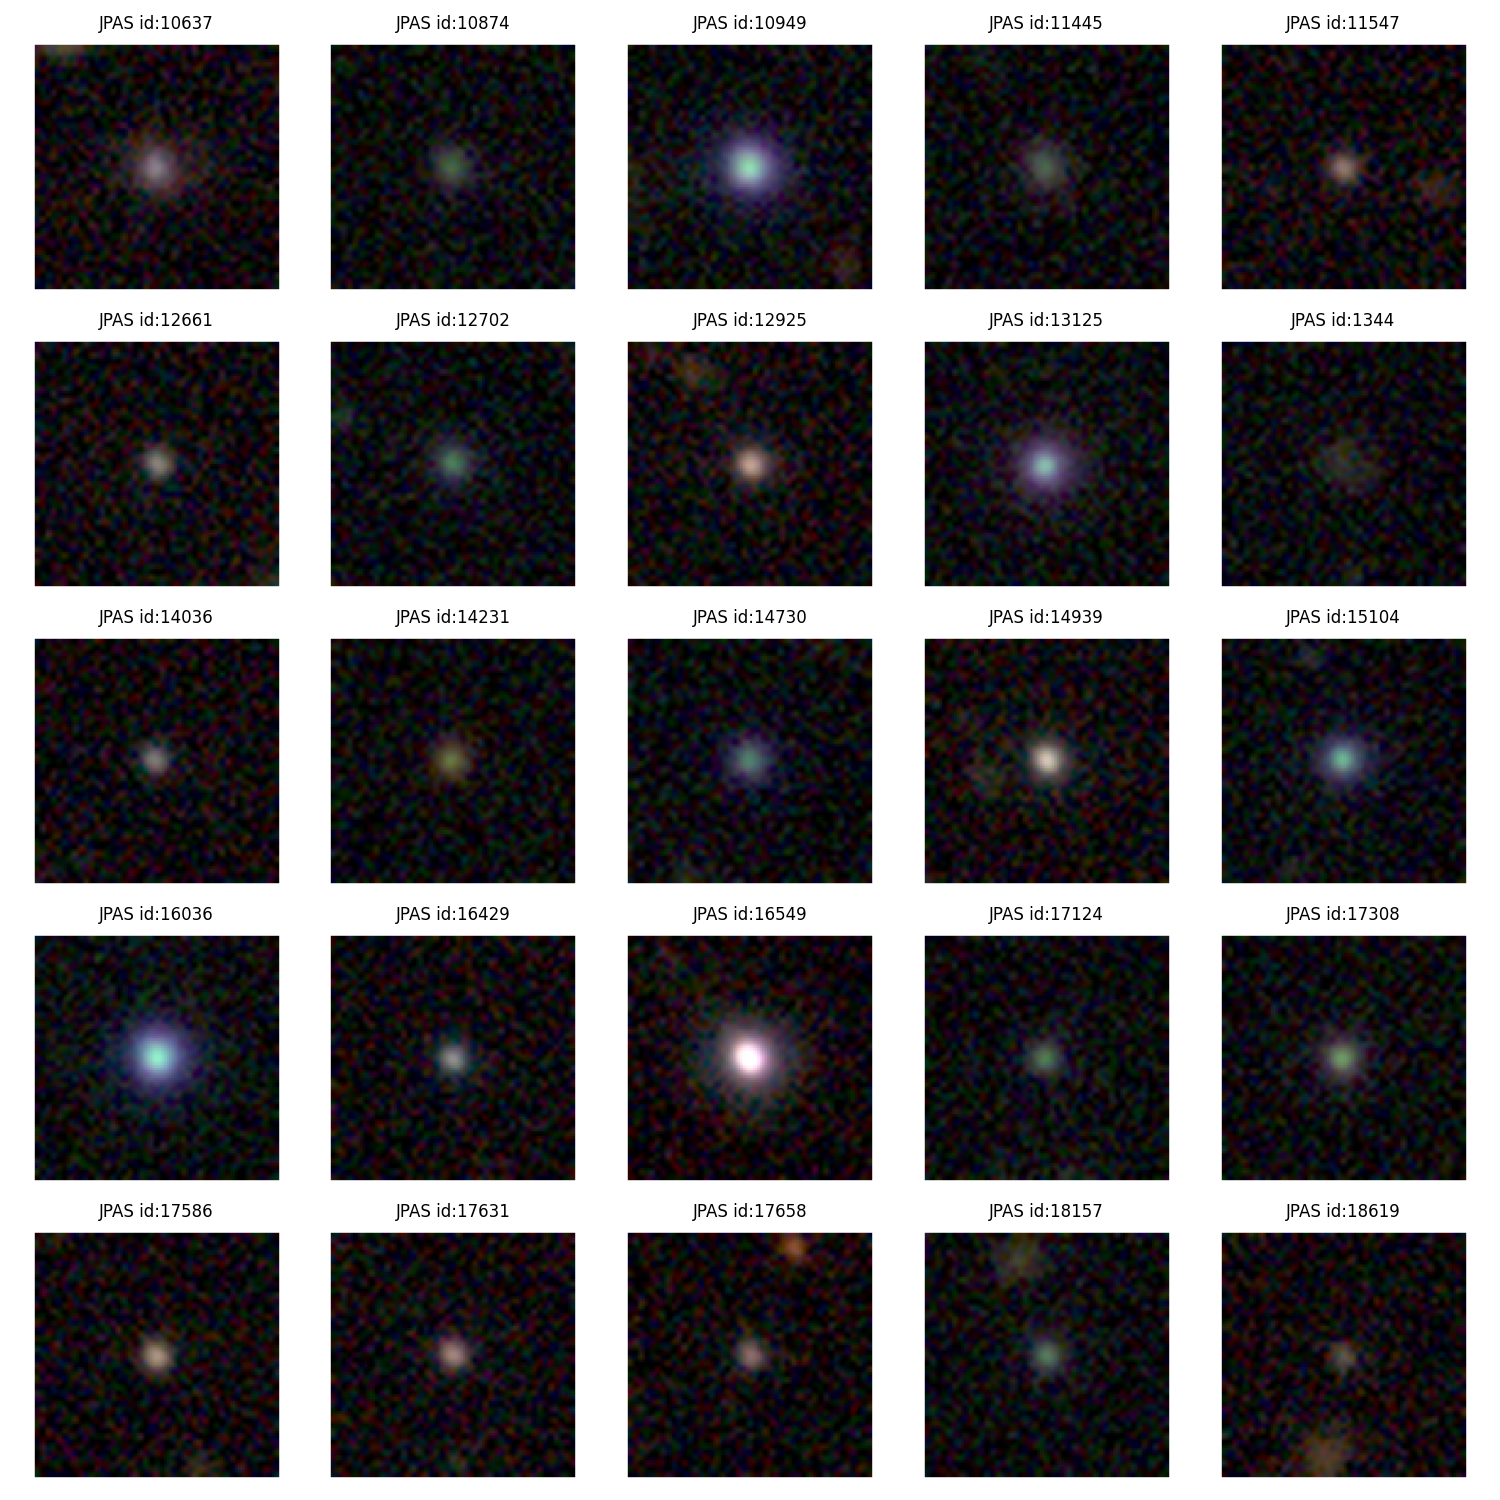
\includegraphics[width=1.0\textwidth]{../../figs/sdss_quasars.png}
        \end{figure}
        \end{columns}
\end{frame}

\begin{frame}
    \frametitle{JPAS vs. SDSS spectra}
    \begin{columns}
        \column{0.5\textwidth}
        \begin{table}
            \caption{SDSS spectra in JPAS-mini}
            \centering
            \begin{tabular}{|c|c|}
                \hline
                Class & Number \\
                \hline
                    GALAXY   & 514 \\
                    STAR     & 238 \\
                    QSO      & 182 \\
                \hline
            \end{tabular}
        \end{table}
        \column{0.5\textwidth}
        \begin{figure}
            \begin{subfigure}{0.75\textwidth}
                \centering
                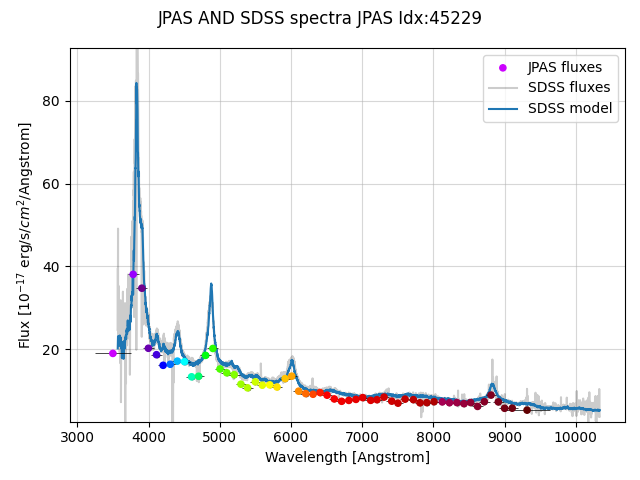
\includegraphics[width=1.0\textwidth]{../../figs/spec/jpas_sdss_45229.png}
            \end{subfigure}
            \pause
            \begin{subfigure}{0.75\textwidth}
                \centering
                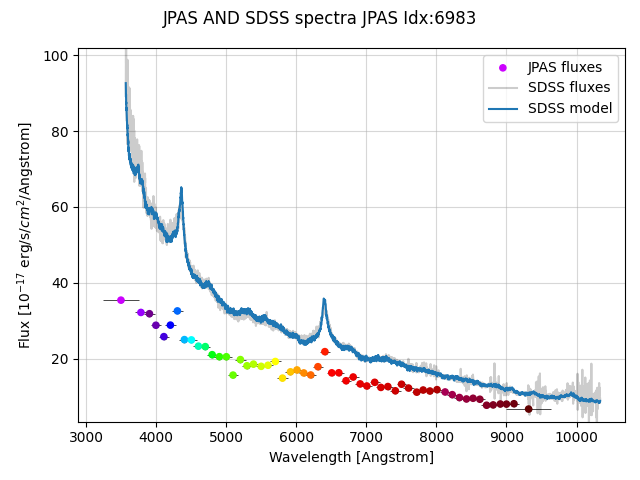
\includegraphics[width=1.0\textwidth]{../../figs/spec/jpas_sdss_6983.png}
            \end{subfigure}
        \end{figure}
        \end{columns}
\end{frame}

\begin{frame}
    \begin{figure}
        \begin{subfigure}{.3\linewidth}
            \centering
            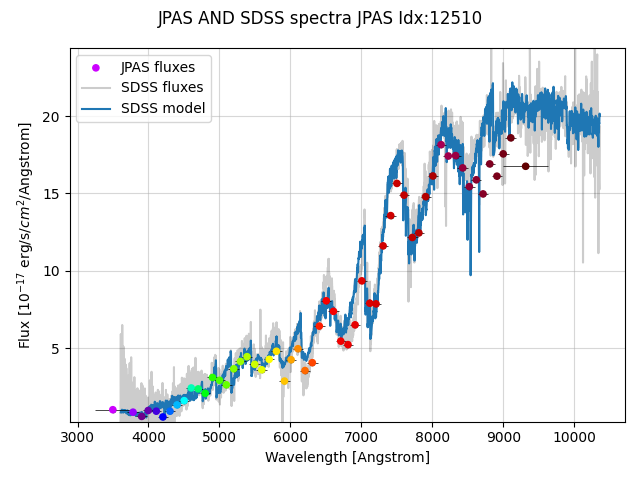
\includegraphics[width=1.0\textwidth]{../../figs/spec/jpas_sdss_12510.png}
        \end{subfigure}
        \begin{subfigure}{0.3\linewidth}
            \centering
            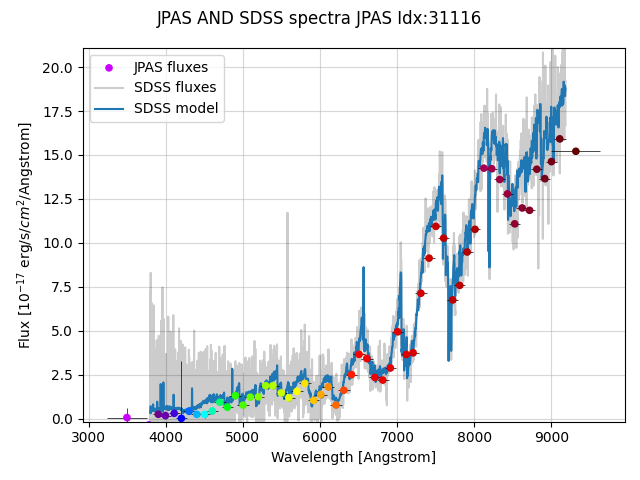
\includegraphics[width=1.0\textwidth]{../../figs/spec/jpas_sdss_31116.png}
        \end{subfigure}
        \begin{subfigure}{0.3\linewidth}
            \centering
            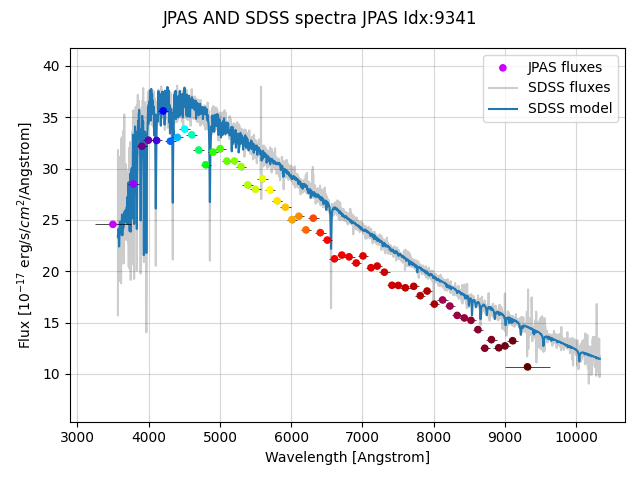
\includegraphics[width=1.0\textwidth]{../../figs/spec/jpas_sdss_9341.png}
        \end{subfigure}
        
        \begin{subfigure}{0.3\linewidth}
            \centering
            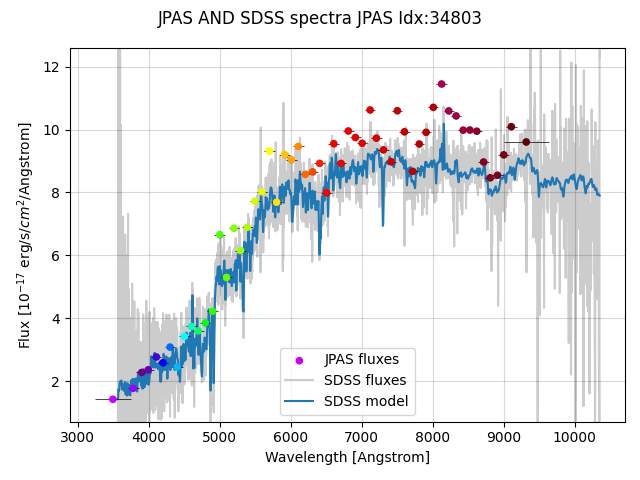
\includegraphics[width=1.0\textwidth]{../../figs/spec/jpas_sdss_34803.png}
        \end{subfigure}
        \begin{subfigure}{0.3\linewidth}
            \centering
            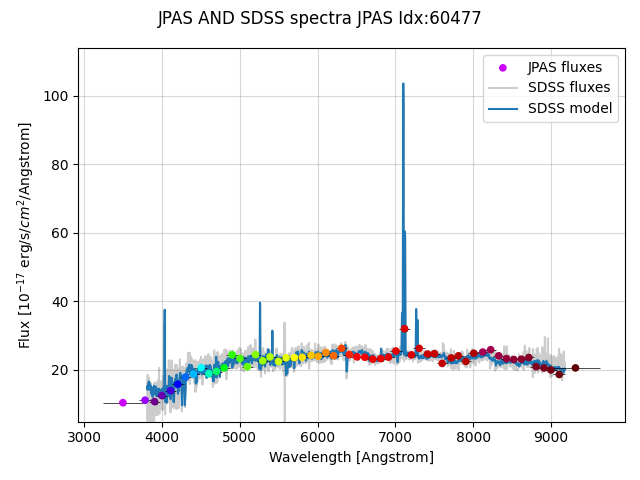
\includegraphics[width=1.0\textwidth]{../../figs/spec/jpas_sdss_60477.png}
        \end{subfigure}
        \begin{subfigure}{0.3\linewidth}
            \centering
            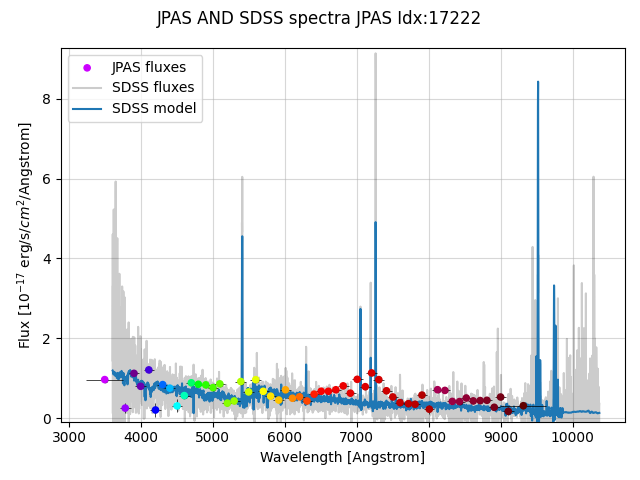
\includegraphics[width=1.0\textwidth]{../../figs/spec/jpas_sdss_17222.png}
        \end{subfigure}

    \end{figure}
\end{frame}

\begin{frame}
    \frametitle{Redshift comparision}
    \begin{columns}
        \column{0.5\textwidth}
        \begin{figure}
            \centering
            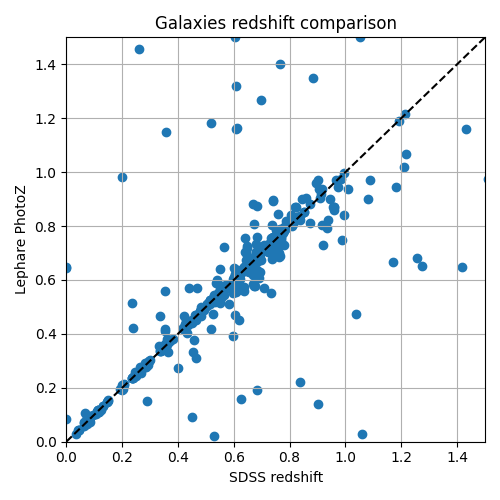
\includegraphics[width=1.0\textwidth]{../../figs/galaxy_redshift_comparison.png}
        \end{figure}
        \pause
        \column{0.5\textwidth}
        \begin{figure}
            \centering
            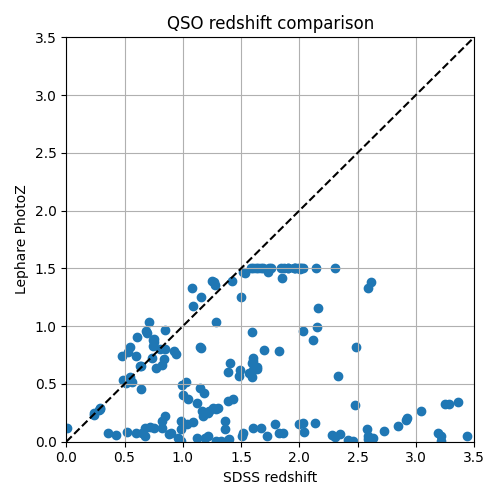
\includegraphics[width=1.0\textwidth]{../../figs/qso_redshift_comparison.png}
        \end{figure}
    \end{columns}
\end{frame}

\section{GAIA sources}

\begin{frame}
    \frametitle{GAIA sources}
    \begin{columns}
        \column{0.5\textwidth}
            GAIA DR3 quasar candidates (6,649,162 sources)
            % gaiadr3.qso_candidates
            % gaiadr3.galaxy_candidates (4,842,342 sources)
        \begin{figure}
            \centering
            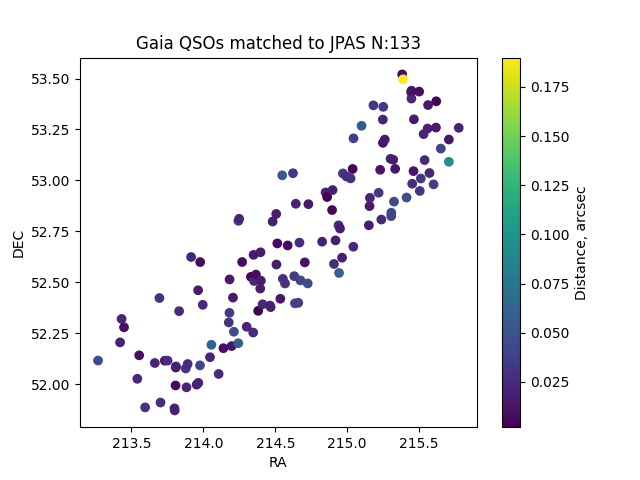
\includegraphics[width=1.0\textwidth]{../../figs/gaia_qso_jpas.png}
        \end{figure}

        No multiplets in the GAIA DR3 quasar candidates in 10 arcsec radius.

        \column{0.5\textwidth}
        \begin{figure}
            \centering
            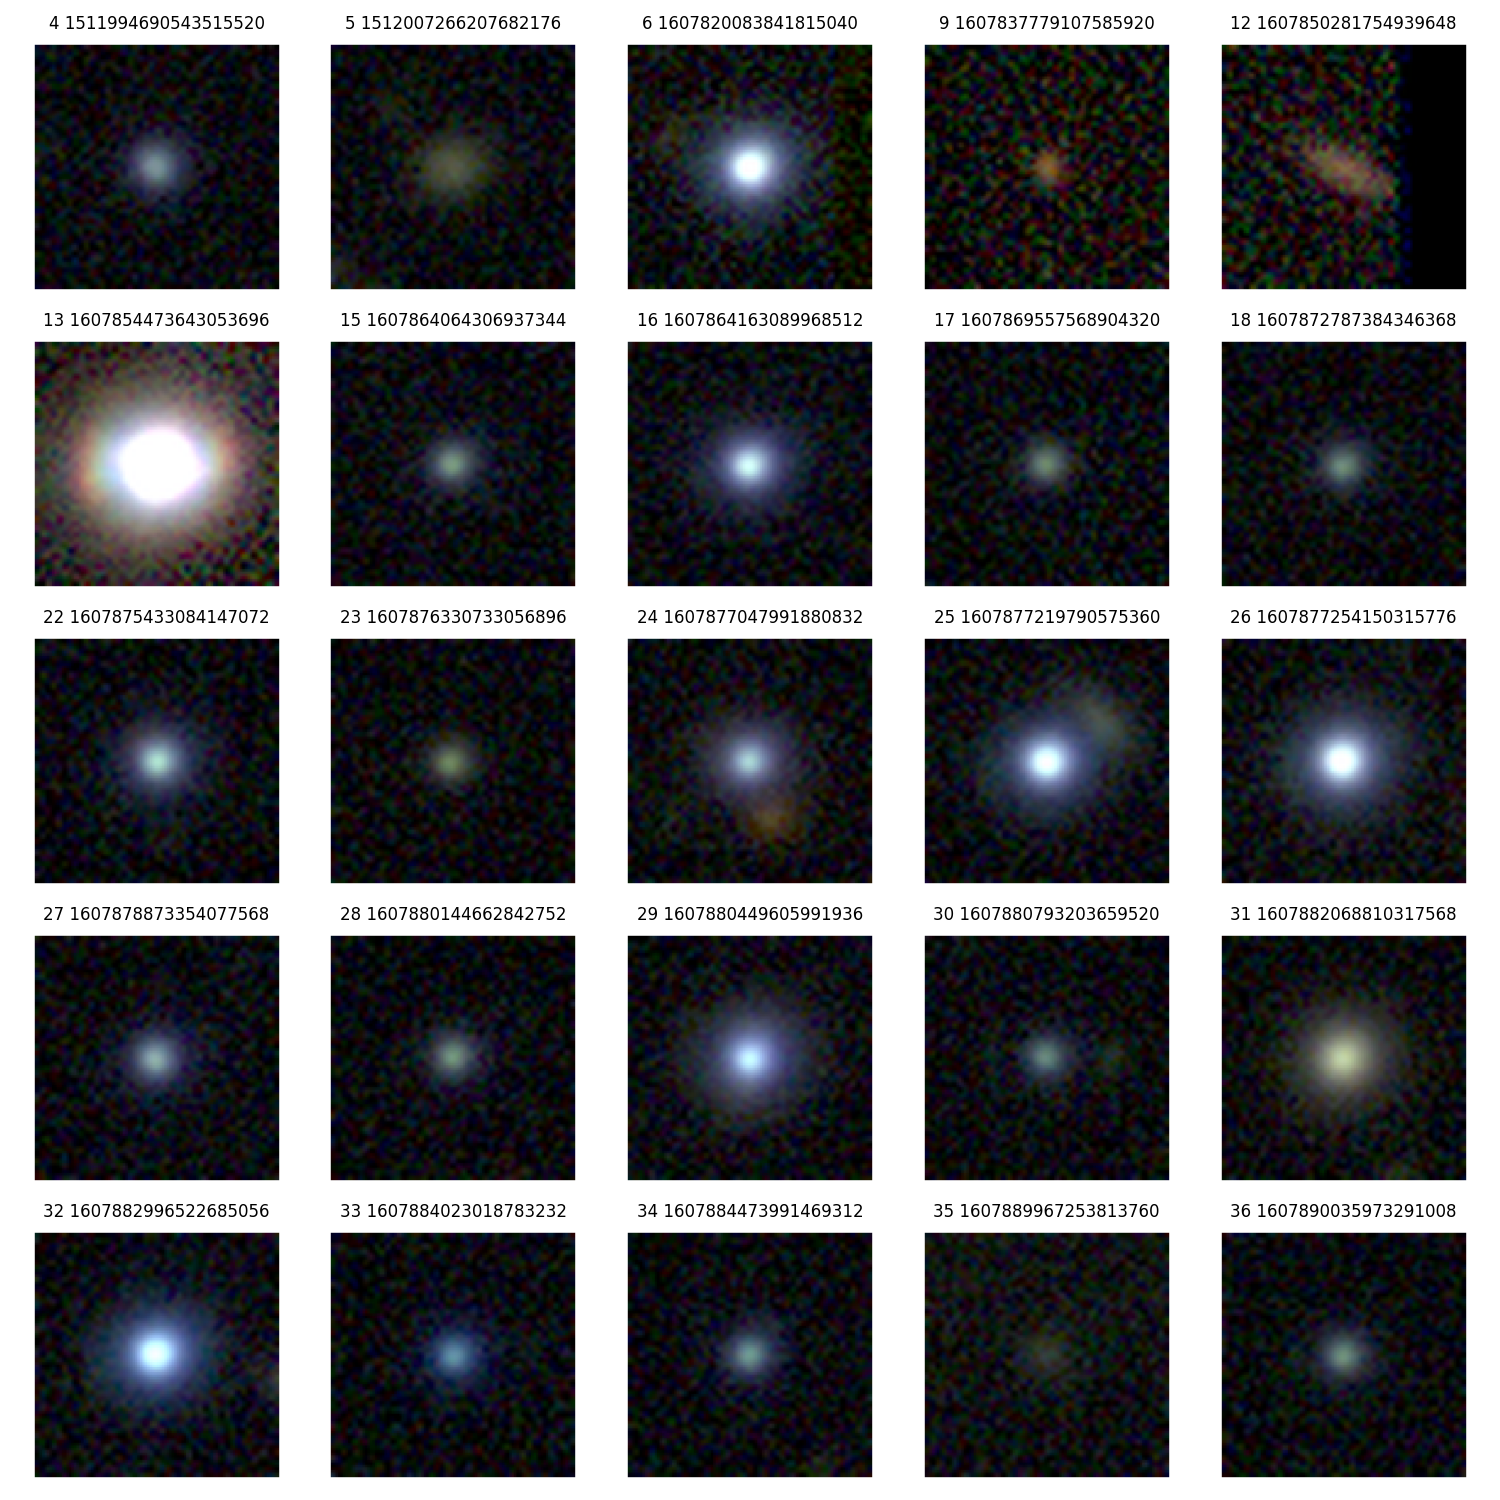
\includegraphics[width=1.0\textwidth]{../../figs/gaia_quasars.png}
        \end{figure}
    \end{columns}
\end{frame}


\begin{frame}
\frametitle{Galaxy-Galaxy lensing}
    Requires a deep learning methods (CNN) to find the lensed sources.
    \begin{columns}
        \column{0.5\textwidth}
        \begin{itemize}
            \item Advantages: More numerous than quasars, have a large number of sources.
            \item Disadvantages: Have a low surface brightness. 
        \end{itemize}
        \column{0.5\textwidth}
        \begin{figure}
            \centering
            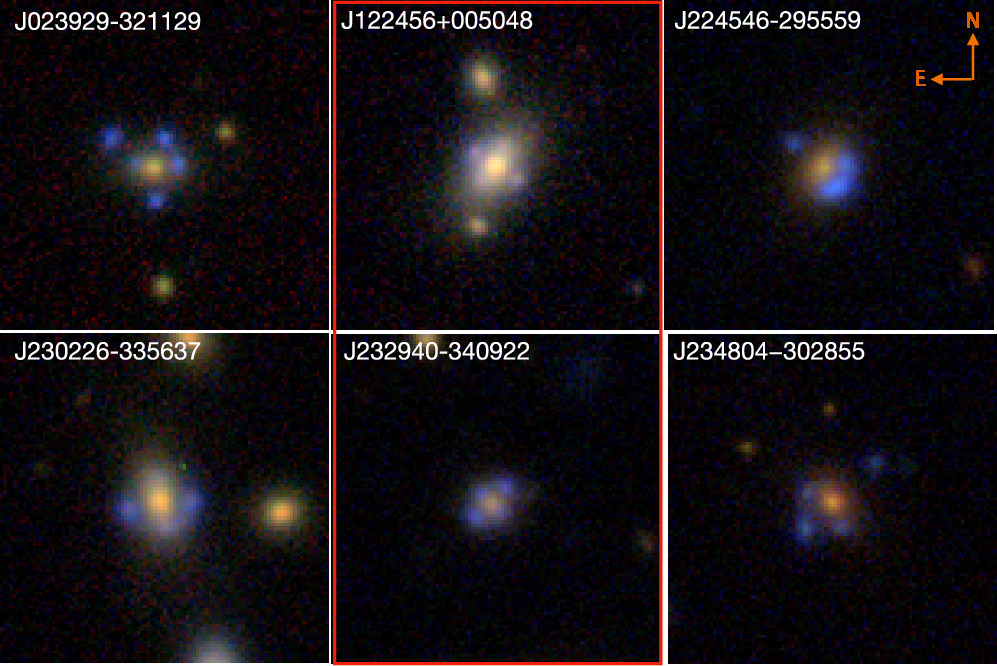
\includegraphics[width=0.8\textwidth]{../../figs/apjad684cf1_lr.jpg}
        \end{figure}
    \end{columns}
        
\end{frame}

\end{document}